\documentclass{article}
\usepackage[utf8]{inputenc}
\usepackage{graphicx}
\usepackage{amsmath}
\usepackage{stmaryrd}   % llbracket, rrbracket
\usepackage{siunitx}	% SI units
\usepackage{geometry}
\usepackage{charter}	% betterfont

\geometry{top=1.5cm,bottom=1.5cm, left=2cm, right=2cm}

\begin{document}

\appendix
\section{Secondary structure elements of an RNA}
RNA secondary structure elements can be classified in stems and loops. Stems are stacks of canonical interactions. They consist in double-stranded regions which stabilize the molecule. \\
Loops are unpaired portions (unpaired in terms of \textit{canonical} pairings) which are often more flexible, and can interact with distant portions of the molecule (forming canonical or non-canonical pseudoknots) or with another molecule, providing a function to the RNA.

\begin{center}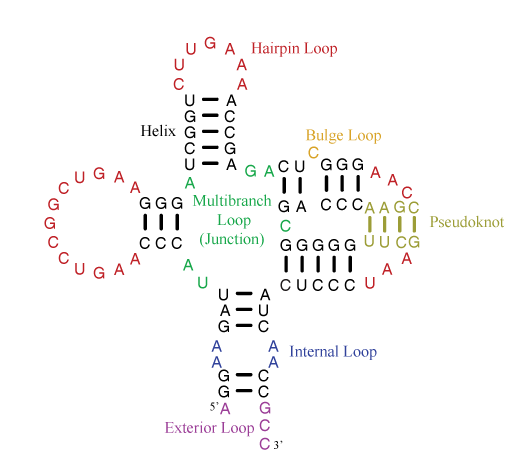
\includegraphics[width=0.5\linewidth]{fig/RNA_SSE.png}\end{center}
\textit{\scriptsize Figure extracted from Dr. Xiang-Jun Lu's 3DNA website (\texttt{https://x3dna.org/articles/exterior-loop-in-rna-secondary-structure}), June 2019}\\

Loops can be further classified according to their number of strands, sometimes called "components" in this article. A \textit{Hairpin Loop} (HL) is composed of only one strand joining the two strands of only one stem. An \textit{Internal Loop} (IL) is composed of two strands linking together two stems. Note that a particular case of IL, called the \textit{bulge}, has one strand of length zero. Loops with more than 2 stems are called \textit{Multibranch Loops} (ML), and sometimes referred as $k$-way junctions for $k$ stems.

The different strands of the loops which link stems together do not necessarily belong to the same RNA molecule, the same vocabulary can be used to describe RNA complexes. For example, if one cuts the top Hairpin Loop on this figure, the bottom Internal Loop remains an Internal Loop, but uses two different RNA molecules. There is no difference from a structural point of view.

\begin{center}
    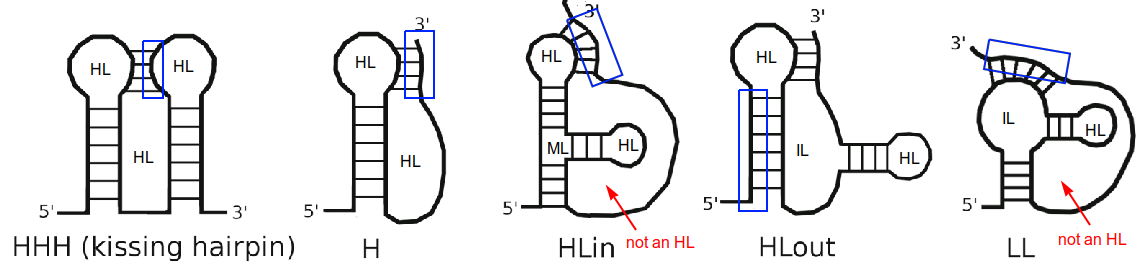
\includegraphics[width=0.8\linewidth]{fig/pseudoknots.png}
\end{center}
Pseudoknots families describe how they can be formed. The HHH type happens when 2 hairpin loops form a new stem together (squared in blue), forming a third hairpin loop. The H type is a simple strand forming a new stem with an HL, forming a new HL. If there is a IL or ML formed instead of a HL, because of a stem+loop already present, we call it a HLin (Hairpin Loop inside the loop). If a strand forms a new stem not with a HL, but with an IL, forming a new HL, we call it a HLout (Hairpin Loop pointing out). If an IL or ML is formed instead of a HL, it is called an LL pseudoknot.

\newpage

%%%%%%%%%%%%%%%%%%%%%%%%%%%%%%%%%%%%%%%%%%%%%%%%%%%%%%%%%%%%%%%%%%%%%%%%%%%%%%%%%%%%%%%
\section{RNA-MoIP can break important base-pairs}
We justify our Pareto-based bi-objective approach by the fact that a linear combination of two objectives (what RNA-MoIP does) always have several defects:
\begin{itemize}
    \item It can miss solutions when the Pareto set is not perfectly convex,
    \item It requires weights on every term of the sum. If these weights are not finely tuned, the compromise between including modules and not breaking important basepairs is missed. We believe this is the case and illustrate this with the following plots:
\end{itemize}

\begin{figure}[h]
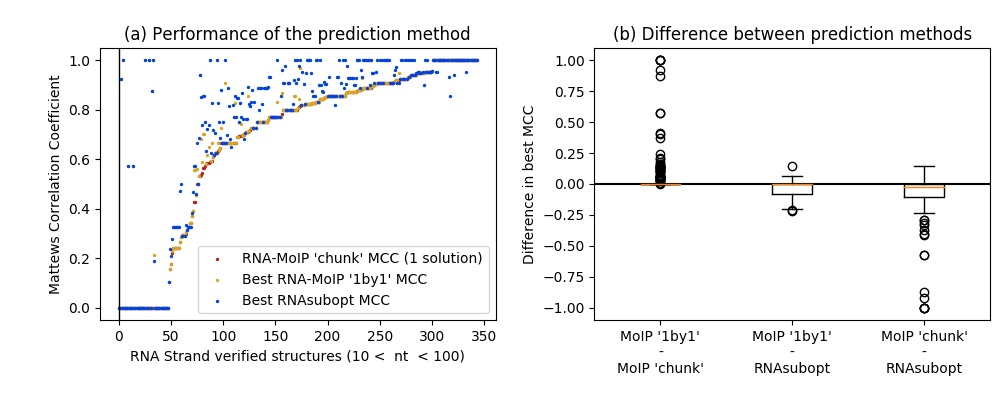
\includegraphics[width=\linewidth]{fig/MOIP_subopt.jpg}
\end{figure}

Here we compare the prediction performance of:
\begin{itemize}
    \item RNAsubopt (which predicts a list of sub-optimal secondary structures without pseudoknots, that are then fed forward into RNA-MoIP), 
    \item RNA-MoIP "chunk", which is the default running mode of RNA-MoIP, which selects only one solution from the list of sub-optimals based on a linear combination of two objectives: the possibility to insert modules with $f_{1A}$ on one side, and not breaking too much basepairs from the input structure on the other side,
    \item RNA-MoIP 'one by one', a different use of RNA-MoIP where we give it every sub-optimal solution one by one and let it modify it to insert modules. Then we manually select the best solution according to max MCC (like we do for RNAsubopt).
\end{itemize}

First on the left figure (a), the max MCC found across the set of solutions is reported for each of the 344 RNAs of the RNA-Strand dataset. RNAs are sorted by RNA-MoIP 'chunk' performance. We can see that the two RNA-MoIP series do not differ a lot, which means RNA-MoIP efficiently selects the best solution in the set after the solutions have been modified to insert modules. But, on the other side, we can see that one of the input RNAsubopt solutions often was better than the solutions transformed by RNA-MoIP: it breaks important basepairs in the inputs.\\
The right figure (b) quantifies the differences. The performance difference between the two RNA-MoIP usages is almost always null, meaning RNA-MoIP is good at selecting its best solution in the set. But when compared to RNAsubopt, the performance decreases more often than it increases.

We think "breaking" base-pairs in an input is not the best way to do, so we chose to build the solutions taking into account the two criteria simultaneously in a bi-objective optimisation program. 

\newpage

%%%%%%%%%%%%%%%%%%%%%%%%%%%%%%%%%%%%%%%%%%%%%%%%%%%%%%%%%%%%%%%%%%%%%%%%%%%%%%%%%%%%%%%
\section{Linear constraints to model RNA Structures in an integer linear program}
We present here the linear constraints we used to model our problem and solve it with a regular integer-linear-programming solver. The constraints have been written by us, but are inspired by works like (Sato \textit{et al.}, 2011), (Reinharz \textit{et al.}, 2012) and (Legendre \textit{et al.}, 2018).

\paragraph{Extended notations} ~ \\
Let $n$ be the number of nucleotides in the query RNA sequence $s$.\\
Let $M$ be the set of modules that could be inserted in $s$.\\
Let $x$ be a module of $M$, $\|x\|$ be the number of distinct components of $x$, and $p(x)$ the associated score of insertion given by JAR3D or BayesPairing for that motif inserted at a particular position.\\
Let $P_{x,i}$ be the position in $s$ where we can insert the $i$th component of module $x$.\\
As the same module model can be inserted several times in $s$, several different $x$ modules in $M$ may refer to the same theoretical module, but inserted at different positions.\\
Let $k_{x,i}$ be the size in nucleotides of that $i$th component of $x$.\\
Let $y^u_v$ be the \textbf{decision boolean variable} indicating that $s[u]$ and $s[v]$ form a canonical base pairing. According to the standard loop model, we always have $v > u + 3$.\\
Let $C^x_i$ be the \textbf{decision boolean variable} indicating that we do insert the $i$th component of module $x$ at position $P_{x,i}$.


Note that a base pair $y^u_v$ is possible if and only if $v>u+3$, and that we do not need to use two variables $y^u_v$ and $y^v_u$ for the same pair. 
Then, we have $\sum_{i=4}^n (n-i)$ decision variables ($\approx \frac{1}{2}n^2$ decision variables) of the form $y^u_v$.
Regarding the $C^x_i$, if we have an average insertion of $\nu$ motifs by RNA sequence, the motifs having in average $\mu$ components, components that can be inserted in average at $\pi$ different positions in $s$,
then we need to add, in average, $\nu \times \mu \times \pi$ decision variables $C^x_i$.

Then, we expect having around $\frac{1}{2}n^2+\nu \mu \pi$ decision variables.

%%%%%%%%%%%%%%%%%%%%%%%%%%%%%%
\paragraph{Constraint to ensure there only is 0 or 1 canonical pairing by nucleotide} ~ 
\begin{equation} \label{constraint:1}
	\sum_{v<u} y^v_u + \sum_{v>u} y^u_v \leq 1 \qquad\qquad \forall u \in \llbracket 1,n \rrbracket
\end{equation}

%%%%%%%%%%%%%%%%%%%%%%%%%%%%%%
\paragraph{Constraints to forbid lonely base pairs} ~
% \begin{equation} \label{constraint:2}
% 	\sum_{v=u}^n y^{u-1}_v - \sum_{v=u+1}^n y^u_v + \sum_{v=u+2}^n y^{u+1}_v \geq 0 \qquad \qquad \forall u \in \llbracket 1,n\rrbracket
% \end{equation}
% \begin{equation} \label{constraint:3}
% 	\sum_{u=1}^{v-2} y^u_{v-1} - \sum_{u=1}^{v-1} y^u_v + \sum_{u=1}^{v} y^u_{v+1} \geq 0 \qquad \qquad \forall v \in \llbracket 1,n\rrbracket
% \end{equation}
% These conditions ensure that if a base pair exists with $s[i]$, 
% one of the adjacent bases is paired too. 
% Equation \ref{constraint:2} is useful if $s[u]$ is paired with $s[v>u]$ (a nucleotide later in the sequence), 
% and equation \ref{constraint:3} if $s[v]$ is paired with $s[u<v]$ (a nucleotide earlier in the sequence).
\begin{equation} \label{constraint:2}
	y^{u-1}_{v+1} - y^u_v + y^{u+1}_{v-1} \geq 0 \qquad \qquad \forall (u,v) \in \{ (u,v) \in \llbracket 1,n\rrbracket^2 \; | \; u + 3 <v \}
\end{equation}
A basepair should be accompanied by one of its neighbours, forming a stable structure stabilized by stacking energies. In theory, this might add up to \( \frac{1}{2}n^2\) constraints, but in practice, this number is very reasonable as
the only decision variables kept are those with probability above a $\theta$ threshold. 
Then, this condition sets to zero "lonely decision variables" who have no neighbour basepair variable allowed.


%%%%%%%%%%%%%%%%%%%%%%%%%%%%%%
% \paragraph{Constraint to forbid pairings inside a module component} ~ 
% \begin{equation} \label{constraint:4}
% 	(k_{x,i}-2) \; C^x_i + \sum_{u=P_{x,i}+1}^{P_{x,i}+k_{x,i}-2}\left[ \sum_{v>u} y^u_v + \sum_{v<u} y^v_u \right] \leq (k_{x,i} - 2)
% 	\qquad \qquad \forall x \in M, i \in \llbracket 1,\|x\| \rrbracket
% \end{equation}
% If $C^x_i$ is set to 1, then the sum has to be zero. Obviously, this constraint prevents the program to correctly detect pseudoknots of HHH (kissing hairpins) and LL types (kissing higher-order loops), which is a limit of the approach.

%%%%%%%%%%%%%%%%%%%%%%%%%%%%%%
\paragraph{Constraints to forbid components to overlap} ~
\begin{equation} \label{constraint:5}
	\sum_{x \in M} \sum_{i=1}^{\|x\|} C^x_i \times I(P_{x,i}<u<P_{x,i}+k_{x,i}-1) \leq 1 \qquad \qquad \forall u \in \llbracket 1,n \rrbracket
\end{equation}
$I(P_{x,i}<u<P_{x,i}+k_{x,i}-1)$ is a boolean value depending on the condition's truth. Then, whatever the nucleotide $u$, it can be part of a module component only once.

%%%%%%%%%%%%%%%%%%%%%%%%%%%%%%
\paragraph{Constraints to respect the structure of large motifs ($\{ x\in M \; | \; \|x\| \geq 2\}$)} ~ 

These constraints ensure that none or all the components of a motif are inserted.
\begin{equation}\label{constraint:6}
	\sum_{i=2}^{\|x\|} C^x_i = (\|x\| - 1) \times C^{x}_{1}	 \qquad \qquad \forall x \in \{ x\in M \; | \; \|x\| \geq 2\}
\end{equation}

And then, we force the base pairs between the end of a component and the beginning of the next one, so that the module $x$ has all its closing basepairs:
\begin{equation}\label{constraint:7}
	C^x_1 \leq y^{P_{x,1}}_{P_{x,\|x\|}+k_{x,\|x\|}-1} \qquad \qquad \forall x \in \{ x\in M \; | \; \|x\| \geq 2\}
\end{equation}
\begin{equation}\label{constraint:8}
	C^x_j \leq y^{P_{x,j}+k_{x,j}-1}_{P_{x,j+1}} \qquad \qquad \forall x \in \{ x\in M \; | \; \|x\| \geq 2\}, \forall j \in \llbracket 1,\|x\| \llbracket
\end{equation}

Constraint (\ref{constraint:7}) binds the first nucleotide of first component to the last one of the last component. 
Constraint (\ref{constraint:8}) binds the last nucleotide of component $j$ to the first of component $j+1$.

%%%%%%%%%%%%%%%%%%%%%%%%%%%%%%
\paragraph{Facultative constraints to forbid pseudoknots} ~
\begin{equation}\label{constraint:9}
	y^u_v + y^k_l \leq 1 \qquad \qquad \forall u,v,k,l \text{ such as } 1\leq u<k<v<l\leq n
\end{equation}

To limit the number of constraints added, we obviously define the condition for allowed basepairs only ($u + 3 <v$, $k + 3 <l$, $p_{uv} > \theta$, $p_{kl} > \theta$).



%%%%%%%%%%%%%%%%%%%%%%%%%%%%%%
\paragraph{Constraints to forbid previously found solutions} ~ 

As several solutions may result in the same values of the two objectives, and as we want to get all the solutions, we can't forbid the algorithm to search twice the same region of the objective space.
We have to explicitly forbid to find again every found solution.\\
We do it by adding iteratively, for every structure $s^*$ found, the following condition:
\begin{equation}\label{constraint:10}
	\sum_{y^u_v \in \{ y^u_v  | y^u_v = 1 \text{ in } s^* \}} (1 - y^u_v) + \sum_{y^u_v \in \{ y^u_v  | y^u_v = 0 \text{ in } s^* \}} y^u_v +
	\sum_{C^x_i \in \{ C^x_i  | C^x_i = 1 \text{ in } s^* \}} (1 - C^x_i) + \sum_{C^x_i \in \{ C^x_i  |C^x_i = 0 \text{ in } s^* \}} C^x_i \geq 1
\end{equation}

It ensures that at least one of the decision variables differs from $s^*$.

\newpage
%%%%%%%%%%%%%%%%%%%%%%%%%%%%%%%%%%%%%%%%%%%%%%%%%%%%%%%%%%%%%%%%%%%%%%%%%%%%%%%%%%%%%%%%%%%%%%%
%%%%%%%%%%%%%%%%%%%%%%%%%%%%%%%%%%%%%%%%%%%%%%%%%%%%%%%%%%%%%%%%%%%%%%%%%%%%%%%%%%%%%%%%%%%%%%%
\section{Case study}

To complete the large benchmark, we have a deeper look at well-known structures to check if some methods are able to predict them correctly. We used a Gln tRNA from E. coli (RNA-Strand code PDB\_00376), a Guanine riboswitch (RNA-Strand code PDB\_01023), and the pseudoknot of the human telomerase (PDB\_00857). The tRNA is unpseudoknotted, the G riboswitch contains a hard-to-predict HHH type pseudoknot, and the telomerase pseudoknot is a simple H type pseudoknot.

%\begin{table}[h]
%\footnotesize{
% \begin{tabular*}{\textwidth}{l@{\extracolsep{\fill}}lllllll}
% \hline 
%   & RNAsubopt & RNA-MoIP & BiokoP &  \multicolumn{4}{c}{BiORSEO}\\
%   & & & & Rna3Dmotif & Rna3Dmotif & 3D Motif Atlas & 3D Motif Atlas\\
%   & & & & + Direct P.M. & + BayesPairing & + JAR3D & + BayesPairing \\
% \hline
%   tRNA Gln & 0.68 & 0.67 & 0.67 &  0.64 (A,B) & 0.64 (B,C,D), 0.60 (A) & 0.64 (B,C,D), 0.63 (B) & 0.64 %(\textit{all}) \\
%   G riboswitch &  0.86 & 0.84, 0.68 & 0.76 & 0.72 (A), 0.15(B) & 0.39 (C,D), 0.15 (A,B) & 0.28 %(\textit{all}) & 0.63 (C,D), 0.57 (A), 0.14 (B)\\
%      Telomerase PK & 0.77 & 0.77, 0.7 & 1.0 &  1.0 & 1.0 (B,C,D), 0.66 (A) & 0.97 (\textit{all}), & 1.0 %(\textit{all})\\
% \hline
% \end{tabular*}
% }
% \end{table}
%The table just above reports the value of the max MCC value found across the Pareto set. Pseudoknots %are allowed. The best structure is often the same across the different objective functions $f_{1A}, %f_{1B}, f_{1C}, f_{1D}$, but the rest of the sets can still differ in number of solutions and diversity. %Detailed results including structures, number of solutions and computation times are provided below. 

The results are consistent with the general benchmark: BiORSEO variants perform slightly worse than Biokop or RNAsubopt.
The tRNA is an example of structure where all methods that support pseudoknots predict some in the loops. On the other hand, the telomerase pseudoknot is correctly predicted by both BiORSEO and Biokop, that support pseudoknots. 

Detailed results are given below for each RNA. The number of unique solutions and computation times are also reported. Note that these cases are small RNAs, resulting in both small number of solutions and small times. The times are the "real" time spent, therefore you should use a 4-thread CPU to reproduce them, because there are several multi-threaded parts in the process. When several tools are required, the times are split by tool (for example, BayesPairing + BiORSEO, or RNAsubopt + JAR3D + BiORSEO). They also are very dependant on the I/O delays. Especially with methods reading modules from disk, you may want to use a very fast storage device (e.g. NVMe SSD NAND storage) to increase the speed.

%%%%%%%%%%%%%%%%%%%%%%%%%%%%%%%%%%%%%%%%%%%%%%%%%%%%%%%%%%%%%%%%%%%%%%%%%%%%%%%%%%%%%%%%%%%%%%%
\subsection{E. coli's Gln tRNA}

\paragraph{Referenced "true" structure in RNA-Strand (PDB 00376)} ~ 

\texttt{GGGGUAUCGCCAAGCGGUAAGGCACCGGAUUCUGAUUCCGGAGGUCGAGGUUCGAAUCCUCGUACCCCAGCCA}

\texttt{((((((..(((.........)))((((((((...))))))))...(((((.......))))))))))).....}

\paragraph{Best prediction results} ~ 

{\scriptsize
\begin{tabular}{rlccl}
Method & Best secondary structure & max MCC & N solutions & time (s)\\
\hline
Reference           & \texttt{((((((..(((.........)))((((((((...))))))))...(((((.......))))))))))).....} & & & \\
RNAsubopt           &    \texttt{(((((((.(((....)))..(((.(((((.......)))))..)))((((.......))))))))))).....} &      0.68  &  4    &   0.0\\
Biokop               &   \texttt{[[[[[[((((...))))...(((.((((([[[....)))))....(((((...]]].)))))]]]]]].))).} &      0.67  &  30   &   634.6\\
RNA-MoIP (1by1)       &  \texttt{((((((..((......))...((.(((((.......)))))..))..((.........))..)))))).....} &      0.67  &  4    &   0.0+9.7\\
RNA-MoIP (chunk)       & \texttt{((((((..((......))...((.(((((.......)))))..))..((.........))..)))))).....} &      0.67  &  1    &   0.0+7.8\\
DESC-Direct P.M.-A            & \texttt{((((((((((...))))...[[[.((((([[[.[[.)))))....(((((]].]]].))))))))))).]]].} &      0.64  &  1    &   9.1\\
DESC-Direct P.M.-B            & \texttt{((((((((((...))))...[[[.((((([[[.[[.)))))....(((((]].]]].))))))))))).]]].} &      0.64  &  3    &   30.1\\
DESC-BPairing-A            &  \texttt{((((((((((...)))....((..((((([[[.[[.))))).{{))((((]].]]].)))))))))))..}}.} &      0.60  &  1    &   103.0-8.9\\
DESC-BPairing-B            &  \texttt{((((((((((...))))...[[[.((((([[[.[[.)))))....(((((]].]]].))))))))))).]]].} &      0.64  &  12   &   103.0-18.6\\
DESC-BPairing-C            &  \texttt{((((((((((...))))...[[[.((((([[[.[[.)))))....(((((]].]]].))))))))))).]]].} &      0.64  &  4     &  103.0-11.1\\
DESC-BPairing-D            &  \texttt{((((((((((...))))...[[[.((((([[[.[[.)))))....(((((]].]]].))))))))))).]]].} &      0.64  &  4     &  103.0+10.6\\
BGSU-BPairing-A            &  \texttt{((((((((((...))))...[[[.((((([[[.[[.)))))....(((((]].]]].))))))))))).]]].} &      0.64  &  5    &   110.9+10.9\\
BGSU-BPairing-B            &  \texttt{((((((((((...))))...[[[.((((([[[.[[.)))))....(((((]].]]].))))))))))).]]].} &      0.64  &  7    &   110.9+10.4\\
BGSU-BPairing-C            &  \texttt{((((((((((...))))...[[[.((((([[[.[[.)))))....(((((]].]]].))))))))))).]]].} &      0.64  &  2    &   110.9+9.5\\
BGSU-BPairing-D            &  \texttt{((((((((((...))))...[[[.((((([[[.[[.)))))....(((((]].]]].))))))))))).]]].} &      0.64  &  2    &   110.9+9.3\\
BGSU-Jar3d-A          &  \texttt{(((((((((((....)))..[[[.((((([[[.[[.))))).)).(((((]].]]].))))))))))).]]].} &      0.63  &  1    &   0.0+1.9+10.3\\
BGSU-Jar3d-B          &  \texttt{((((((((((...))))...[[[.((((([[[.[[.)))))....(((((]].]]].))))))))))).]]].} &      0.64  &  1     &  0.0+1.9+9.8\\
BGSU-Jar3d-C          &  \texttt{((((((((((...))))...[[[.((((([[[.[[.)))))....(((((]].]]].))))))))))).]]].} &      0.64  &  2    &   0.0+1.9+10.4\\
BGSU-Jar3d-D          &  \texttt{((((((((((...))))...[[[.((((([[[.[[.)))))....(((((]].]]].))))))))))).]]].} &      0.64  &  2    &   0.0+1.9+10.5\\
\end{tabular}}

\paragraph{Notes} ~

Note that both BiORSEO and BiokoP insert a false-positive pseudoknot. If we look at our recommended method, Rna3Dmotifs + Direct Pattern-matching  + $f_{1A}$, here is an example of difference in the number of solutions : Biorseo returns 1 solution in 9.1s, while others return more solution in longer times, without doing better.

%%%%%%%%%%%%%%%%%%%%%%%%%%%%%%%%%%%%%%%%%%%%%%%%%%%%%%%%%%%%%%%%%%%%%%%%%%%%%%%%%%%%%%%%%%%%%%%
\subsection{G Riboswitch}

\paragraph{Referenced "true" structure in RNA-Strand (PDB 01023)} ~ 

\texttt{GGACAUACAAUCGCGUGGAUAUGGCACGCAAGUUUCUGCCGGGCACCGUAAAUGUCCGACUAUGUCCA}

\texttt{(((((((...(((((((.[[..[[)))))))........((((((]]...]]))))))..))))))).}

\paragraph{Best prediction results} ~ 

{\scriptsize
\begin{tabular}{rlccl}
Method & Best secondary structure & max MCC & N solutions & time (s)\\
\hline
Reference               &\texttt{(((((((...(((((((.[[..[[)))))))........((((((]]...]]))))))..))))))).} & & & \\
RNAsubopt               &\texttt{(((((((.....(((((.......)))))..........((((((.......))))))..))))))).} &   0.86  &  3   &    0.0 \\
Biokop                  &\texttt{(((((((.[[(([[[[[))(((((]]]]]..((]]..))[[[[[[)))))..]]]]]]..))))))).} &   0.76  &  14  &    330.9\\
RNA-MoIP (1by1)         &\texttt{(((((((.....(((((.......)))))..........(((((.........)))))..))))))).} &   0.84  &  3&       0.0+4.6\\
RNA-MoIP (chunk)        &\texttt{(((((((........((.......)).....((....)).((((.........))))...))))))).} &   0.68  &  1&       0.0+3.3\\
DESC-Direct P.M.-A             &\texttt{((((((((....(((((.....[[)))))..((....))[[[[[[..))...]]]]]].]])))))).} &   0.72  &  1 &      6.5\\
DESC-Direct P.M.-B             &\texttt{((((((......(((([[[[[[[[.))))..((((.[[[.))))...]]].))))))..]]]]]]]].} &   0.15  &  7 &      8.4\\
DESC-BPairing-A              &\texttt{((((((((.((.(((([[[[[[[[.))))..))((.[[[.))]]]..))..))))))..]]]]]]]].} &   0.15  &  2 &      91.2+5.6\\
DESC-BPairing-B              &\texttt{((((((((.((.(((([[[[[[[[.))))..))((.[[[.))]]]..))..))))))..]]]]]]]].} &   0.15  &  2 &      91.2+5.8\\
DESC-BPairing-C              &\texttt{(((([[((....((....{{..[[.[[))..]]...((([[[)))..))....))]]].]]]]}})).} &   0.39  &  7  &     91.2+8.6\\
DESC-BPairing-D              &\texttt{(((([[((....((....{{..[[.[[))..]]...((([[[)))..))....))]]].]]]]}})).} &   0.39  &  7 &      91.2+8.5\\
BGSU-BPairing-A              &\texttt{((..(((((((..((((.[[..[[))))[[.)))..]].[[[[[[..))...]]]]]].]]))]])).} &   0.57  &  1  &     102.3+6.6\\
BGSU-BPairing-B              &\texttt{(((((((((((.(((([[[[[[[[.))))..)))..(((.[[)))]]))..))))))..]]]]]]]].} &   0.14  &  2  &     102.3+6.2\\
BGSU-BPairing-C              &\texttt{((..((((....(((((.[[..[[)))))..((....))[[[[[[..))...]]]]]].]]))]])).} &   0.63  &  3  &     102.3+14.0\\
BGSU-BPairing-D              &\texttt{((..((((....(((((.[[..[[)))))..((....))[[[[[[..))...]]]]]].]]))]])).} &   0.63  &  4  &     102.3+7.3\\
BGSU-Jar3d-A            &\texttt{(((..((.....((((([[[[[[[)))))..((....))(((.[[)))))..]])))..]]]]]]]..} &   0.28  &  5  &     0.0+1.5+25.6\\
BGSU-Jar3d-B            &\texttt{(((..((.....((((([[[[[[[)))))..((....))(((.[[)))))..]])))..]]]]]]]..} &   0.28  &  5  &     0.0+1.5+30.6\\
BGSU-Jar3d-C            &\texttt{(((..((.....((((([[[[[[[)))))..((....))(((.[[)))))..]])))..]]]]]]]..} &   0.28  &  6  &     0.0+1.5+7.4\\
BGSU-Jar3d-D            &\texttt{(((..((.....((((([[[[[[[)))))..((....))(((.[[)))))..]])))..]]]]]]]..} &   0.28  &  6  &     0.0+1.5+7.3\\

\end{tabular}}

\paragraph{Notes} ~

Here is a good example showing that MCC does not reflects the correct prediction of pseudoknots. The reference structure contains a small HHH-type knot between the two main hairpin loops, with an additional stem, itself containing an internal loop. Biokop finds it. The BiORSEO variants don't, most of them find other H-type pseudoknots, which all are wrong from a RNA function point of view, but the MCC scores are very diverse even if the structure is wrong, because the basepair lists can share a various amount of positives with the reference even if not located in the same stems. For example, Rna3Dmotifs + Direct Pattern-matching + $f_{1A}$ is at least able to identify the two hairpin loops, its score is much greater than the others (0.72), and the pseudoknot is still wrong.


%%%%%%%%%%%%%%%%%%%%%%%%%%%%%%%%%%%%%%%%%%%%%%%%%%%%%%%%%%%%%%%%%%%%%%%%%%%%%%%%%%%%%%%%%%%%%%%
\subsection{Human telomerase's RNA pseudoknot}

\paragraph{Referenced "true" structure in RNA-Strand (PDB 00857)} ~ 

\texttt{GGGCUGUUUUUCUCGCUGACUUUCAGCCCCAAACAAAAAAGUCAGCA}

\texttt{[[[[[[........(((((((((]]]]]]........))))))))).}

\paragraph{Best prediction results} ~ 

{\scriptsize
\begin{tabular}{rlccl}
Method & Best secondary structure & max MCC & N solutions & time (s)\\
\hline
Reference       &        \texttt{[[[[[[........(((((((((]]]]]]........))))))))).} & & & \\
RNAsubopt       &        \texttt{..............(((((((((..............))))))))).} & 0.77  &  3    &   0.0 \\
Biokop          &        \texttt{[[[[[[........(((((((((]]]]]]........))))))))).} & 1.00  &  1    &   2.4\\
RNA-MoIP (1by1) &        \texttt{..............(((((((((..............))))))))).} & 0.77  &  3    &   0.0 + 2.1\\
RNA-MoIP (chunk)&        \texttt{((..........))(((((((((..............))))))))).} & 0.70  &  1    &   0.0 + 1.0\\
DESC-Direct P.M.-A     &        \texttt{[[[[[[........(((((((((]]]]]]........))))))))).} & 1.00  &  1    &   0.8\\
DESC-Direct P.M.-B     &        \texttt{[[[[[[........(((((((((]]]]]]........))))))))).} & 1.00  &  1    &   0.9\\
DESC-BPairing-A      &        \texttt{[[[[[[........(((((((((]]].]]]......)).))))))).} & 0.66  &  1    &   63.9+0.7\\
DESC-BPairing-B      &        \texttt{[[[[[[........(((((((((]]]]]]........))))))))).} & 1.00  &  2    &   63.9+0.8\\
DESC-BPairing-C      &        \texttt{[[[[[[........(((((((((]]]]]]........))))))))).} & 1.00  &  2    &   63.9+0.7\\
DESC-BPairing-D      &        \texttt{[[[[[[........(((((((((]]]]]]........))))))))).} & 1.00  &  2    &   63.9+0.7\\
BGSU-BPairing-A      &        \texttt{[[[[[[........(((((((((]]]]]]........))))))))).} & 1.00  &  2    &   73.1+0.7\\
BGSU-BPairing-B      &        \texttt{[[[[[[........(((((((((]]]]]]........))))))))).} & 1.00  &  2    &   73.1+0.7\\
BGSU-BPairing-C      &        \texttt{[[[[[[........(((((((((]]]]]]........))))))))).} & 1.00  &  2    &   73.1+0.7\\
BGSU-BPairing-D      &        \texttt{[[[[[[........(((((((((]]]]]]........))))))))).} & 1.00  &  2    &   73.1+0.7\\
BGSU-Jar3d-A    &        \texttt{[[[[[[........((((((((.]]]]]].........)))))))).} & 0.97  &  1    &   0.0+1.7+0.7\\
BGSU-Jar3d-B    &        \texttt{[[[[[[........((((((((.]]]]]].........)))))))).} & 0.97  &  1    &   0.0+1.7+0.8\\
BGSU-Jar3d-C    &        \texttt{[[[[[[........((((((((.]]]]]].........)))))))).} & 0.97  &  1    &   0.0+1.7+0.7\\
BGSU-Jar3d-D    &        \texttt{[[[[[[........((((((((.]]]]]].........)))))))).} & 0.97  &  1    &   0.0+1.7+0.7\\
\end{tabular}}


\paragraph{Notes} ~

The methods which support pseudoknots are able to predict it correctly.

\newpage
%%%%%%%%%%%%%%%%%%%%%%%%%%%%%%%%%%%%%%%%%%%%%%%%%%%%%%%%%%%%%%%%%%%%%%%%%%%%%%%%%%%%%%%%%%%%%%%
%%%%%%%%%%%%%%%%%%%%%%%%%%%%%%%%%%%%%%%%%%%%%%%%%%%%%%%%%%%%%%%%%%%%%%%%%%%%%%%%%%%%%%%%%%%%%%%
\section{Average MCC of the method's variants}
Instead of looking at the max MCC to see if the reference structure has been found in the Pareto set, one can look at the average MCC over the Pareto set.

We provide such results to satisfy the reader's curiosity, but this average is hard to interpret. 
The Pareto set is supposed to propose several solutions that could be several meta-stable states, but there is no reason that these states should be close one to another, nor to be close to the "true" structure that has been observed and saved in the database.
A possible interpretation is the average distance of the meta-stable states to the "true" structure, if and only if we assume the predictions are correct.
It also gives the user an idea of how close to a real conformation he is if he chooses a structure randomly in the Pareto set.

\vspace{0.5cm}
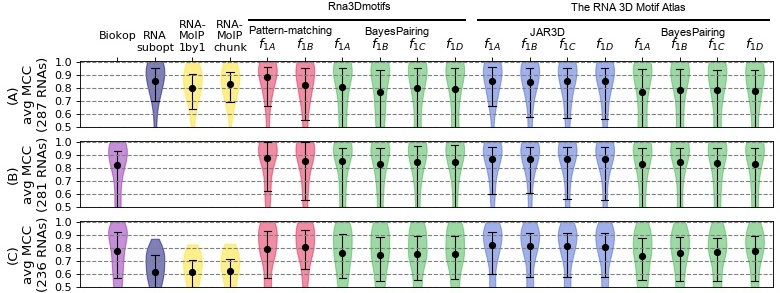
\includegraphics[width=0.95\textwidth]{fig/Benchmark_avg.jpg}
\vspace{0.5cm}

Average MCC obtained by the different methods considered in our benchmark. On (A), the RNAstrand dataset for methods which do not support pseudoknots (computations succeeded for all methods for 287 RNAs). (B) is the same dataset but with pseudoknot support (281 RNAs), and (C) is the Pseudobase dataset, with 236 RNAs.


\newpage
%%%%%%%%%%%%%%%%%%%%%%%%%%%%%%%%%%%%%%%%%%%%%%%%%%%%%%%%%%%%%%%%%%%%%%%%%%%%%%%%%%%%%%%%%%%%%%%
%%%%%%%%%%%%%%%%%%%%%%%%%%%%%%%%%%%%%%%%%%%%%%%%%%%%%%%%%%%%%%%%%%%%%%%%%%%%%%%%%%%%%%%%%%%%%%%
\section{Positions of the best solutions in Pareto sets}
Here we report the position of the best solution (the one which has the max MCC with the true structure) in the normalized Pareto set. The normalization consists in dividing the objective functions values of a solution by the maximum value observed in the Pareto set on each axis. Then, 0 on an axis is the value 0 of the objective, and 1 is the maximum value observed.
The first line is identical to Figure 6. Direct P.M.-$f_{1A}$, Direct P.M.-$f_{1B}$, Jar3d-$f_{1A}$ and Jar3d-$f_{1B}$ are the variants that sometimes result in combinatorial issues.

\begin{figure}[h!]
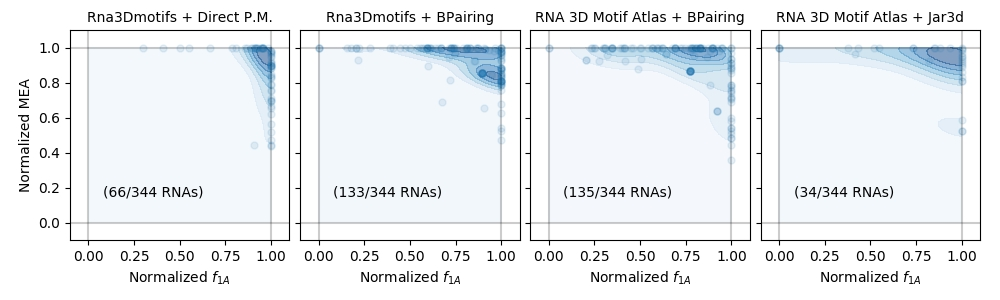
\includegraphics[width=\textwidth]{kernels_A.jpg}
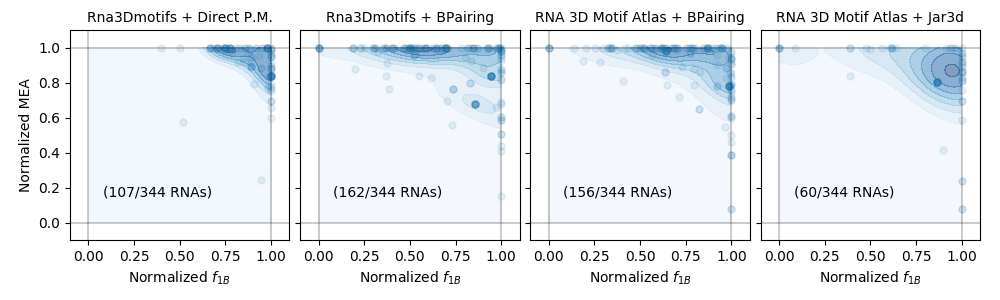
\includegraphics[width=\textwidth]{fig/kernels_B.png}
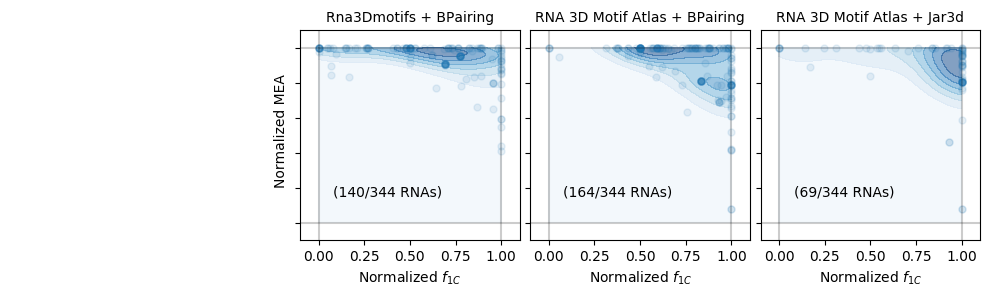
\includegraphics[width=\textwidth]{fig/kernels_C.png}
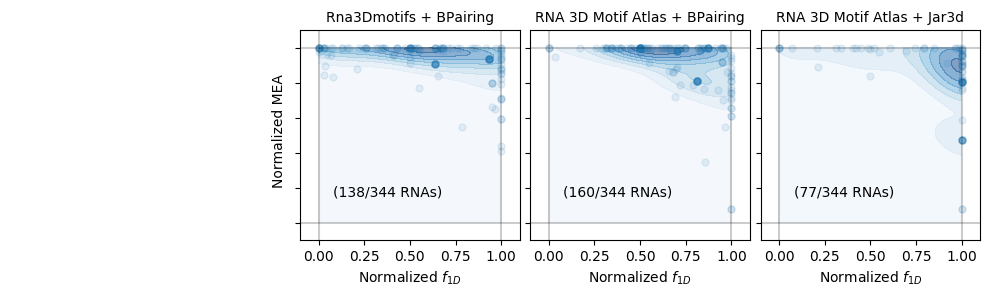
\includegraphics[width=\textwidth]{fig/kernels_D.png}
\end{figure}

\end{document}